\section{Detector-aware phase training and combined gains}

\subsection{Training the measurement signatures rather than raw speckle statistics}

The final phase-training direction retained a single plate but changed the objective. Instead of optimising only illumination statistics, it formed voxel-integrated measurement vectors through the actual emission optics and detector. At sampled lateral positions, the 16 depth-voxel columns were centred and normalised, then their off-diagonal correlations were penalised:
\[
\mathcal L=\mathbb E_{(x,y)}\left[
\frac{\sum_{i\ne j}w_{ij}
\left(\widetilde{\mathbf a}_i^\top\widetilde{\mathbf a}_j\right)^2}
{\sum_{i\ne j}w_{ij}}\right].
\]
Here \(\widetilde{\mathbf a}_i\) is the centred, unit-norm measurement vector for depth voxel i at the sampled lateral position; \(w_{ij}\) doubles selected mirror pairs. Training used 600 Adam iterations, learning rate 0.05, 24 lateral positions and eight directions per step, starting from the reference random plate. The loss is scale-free and contains no specimen-specific reconstruction target. It is detector-aware training, not end-to-end training through the learned solver.

At NA 0.1/12\ensuremath{\times}12, mean absolute depth correlation fell from about 0.855 to 0.543. At NA 0.3/48\ensuremath{\times}48 it fell from about 0.83 to 0.50. The worst correlated pair remained near one, so training did not eliminate every ambiguous direction.

\subsection{Original detector: a reproducible improvement}

The table below uses the final detector/plate block, one noise realisation per subvolume and independently tuned solvers. It should not be substituted into the earlier three-realisation solver table.

\par\medskip\noindent\begin{minipage}{\linewidth}
\captionof{table}{Random and trained plates at NA 0.1 with a 12$\times$12 detector. Values are PSNR (dB) / depth error (micrometres).}
\centering
\begin{tabular}{@{}>{\raggedright\arraybackslash}p{0.227500\linewidth}@{\hspace{0.03\linewidth}}>{\raggedright\arraybackslash}p{0.227500\linewidth}@{\hspace{0.03\linewidth}}>{\raggedright\arraybackslash}p{0.227500\linewidth}@{\hspace{0.03\linewidth}}>{\raggedright\arraybackslash}p{0.227500\linewidth}@{}}\toprule
Plate & Generic prior, C=1: PSNR / depth & Learned prior, C=1: PSNR / depth & Learned prior, C=8: PSNR / depth \\
\midrule
Random 0 & 31.61 / 0.497 & 33.19 / 0.346 & 32.09 / 0.475 \\
Random 1 & 31.58 / 0.495 & 33.17 / 0.354 & 32.10 / 0.506 \\
Random 2 & 31.60 / 0.487 & 33.14 / 0.348 & 32.12 / 0.474 \\
Trained & 32.85 / 0.366 & 34.36 / 0.277 & 33.04 / 0.388 \\
Trained repeat & --- & 34.44 / 0.279 & 33.05 / 0.383 \\
\bottomrule\end{tabular}
\end{minipage}\par\medskip


PSNR is in dB and depth error in \ensuremath{\mu}m. Against each random plate, the trained plate improved PSNR in all eight subvolumes for both solvers at full and eight-fold-compressed measurements. Depth improved in all eight except two generic-prior compressed comparisons with seven improvements. A second training run reproduced the result. Random-plate variation was much smaller than the trained-versus-random mean gain.

Training also improved recovery with the generic prior, so the result was not dependent on the new learned decoder. Against random plate 0 at full measurements, the generic-prior paired depth change was −0.131±0.068 \ensuremath{\mu}m; with the learned prior it was −0.069±0.036 \ensuremath{\mu}m. This is the main successful validation of the detector-aware proxy against actual reconstruction.


\begin{figure}[htbp]
\centering
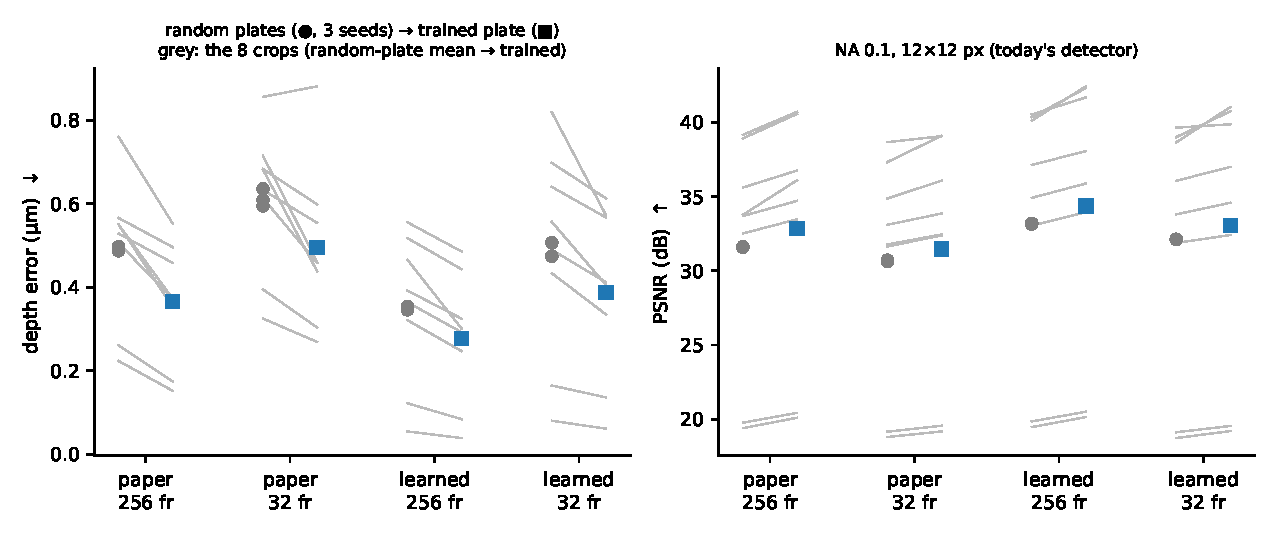
\includegraphics[width=\linewidth,height=0.48\textheight,keepaspectratio]{figures/learned_plate.pdf}
\caption{Detector-aware training versus three random plates at NA 0.1 and a 12$\times$12 detector, with generic and learned priors at 256 and 32 images. Grey lines connect each subvolume's random-plate mean to its trained-plate result. Original final-package plot.}
\label{exp:fig_trained_vs_random_plate}
\end{figure}
\FloatBarrier
\subsection{Higher NA: a mixed result and an untested direction}

At NA 0.3/48\ensuremath{\times}48, a plate trained for 16 images reduced mean depth error from 0.314 to 0.274 \ensuremath{\mu}m, improving six of eight subvolumes. Mean PSNR decreased by about 0.45 dB, largely because of one sparse crop. At two images, outside the training condition, depth error worsened from 0.834 to 1.176 \ensuremath{\mu}m. This is not a clean improvement at high NA, and it does not establish a successful two-image system.

\subsection{Encoder and prior improvements can combine}

At the original detector, trained plate plus learned prior with 32 images achieved 33.04 dB and 0.388 \ensuremath{\mu}m, compared with random plate plus generic prior with 256 images at 31.61 dB and 0.497 \ensuremath{\mu}m. The paired depth difference was −0.109±0.100 \ensuremath{\mu}m, improving six of eight subvolumes; PSNR improved in five of eight. The mean advantage therefore stacks, but it is not a uniform per-subvolume win against that cross-compression reference.

\textbf{Conclusion:} detector-aware phase training succeeds where earlier field-statistics losses were inconclusive. The useful objective acts on the measurement signatures that reconstruction actually receives. Its success at the original detector does not automatically transfer to higher NA or fewer training directions.

Evidence: D25; {\small\texttt{train\_\allowbreak{}detector\_\allowbreak{}aware.\allowbreak{}py}}; final {\small\texttt{designs/\allowbreak{}}}, plate block and paired comparisons.


\begin{figure}[htbp]
\centering
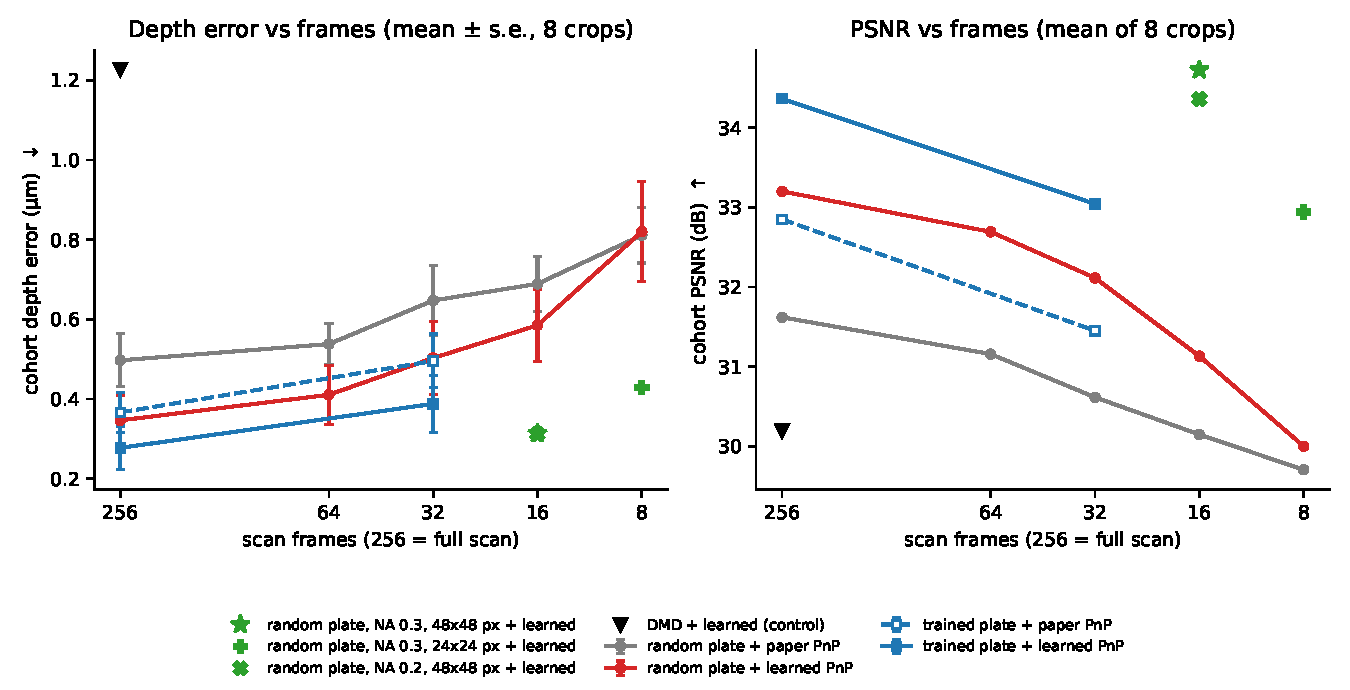
\includegraphics[width=\linewidth,height=0.48\textheight,keepaspectratio]{figures/compression.pdf}
\caption{Observed recovery across encoder, prior and detector changes. The horizontal axis is camera-image count, not a common compression factor across detector sizes. Depth-error bars show standard errors across eight subvolumes, whereas tables in this record report means or sample standard deviations. This is an empirical comparison, not a proven optimal frontier.}
\label{exp:fig_compression_frontier}
\end{figure}
\FloatBarrier
